\chapter{Diseño e implementación} % Main chapter title

\label{Chapter3} % Change X to a consecutive number; for referencing this chapter elsewhere, use \ref{ChapterX}
%----------------------------------------------------------------------------------------
%	ADQUISICION DE DATOS
%----------------------------------------------------------------------------------------
\section{Adquisición de datos}
 
\newcommand{\myhash}{\raisebox{\depth}{\#}}

Para llevar a cabo el presente trabajo, se emplearon datos proporcionados por el servicio 
de cardiología e hipertensión del Hospital Alemán. La figura \ref{fig:adquisicion_datos} 
exhibe un diagrama en bloques que ilustra la etapa de adquisición de datos utilizada. 
Es importante destacar que se utilizaron dos conjuntos de datos diferentes. 

\begin{figure}[ht]
	\centering
	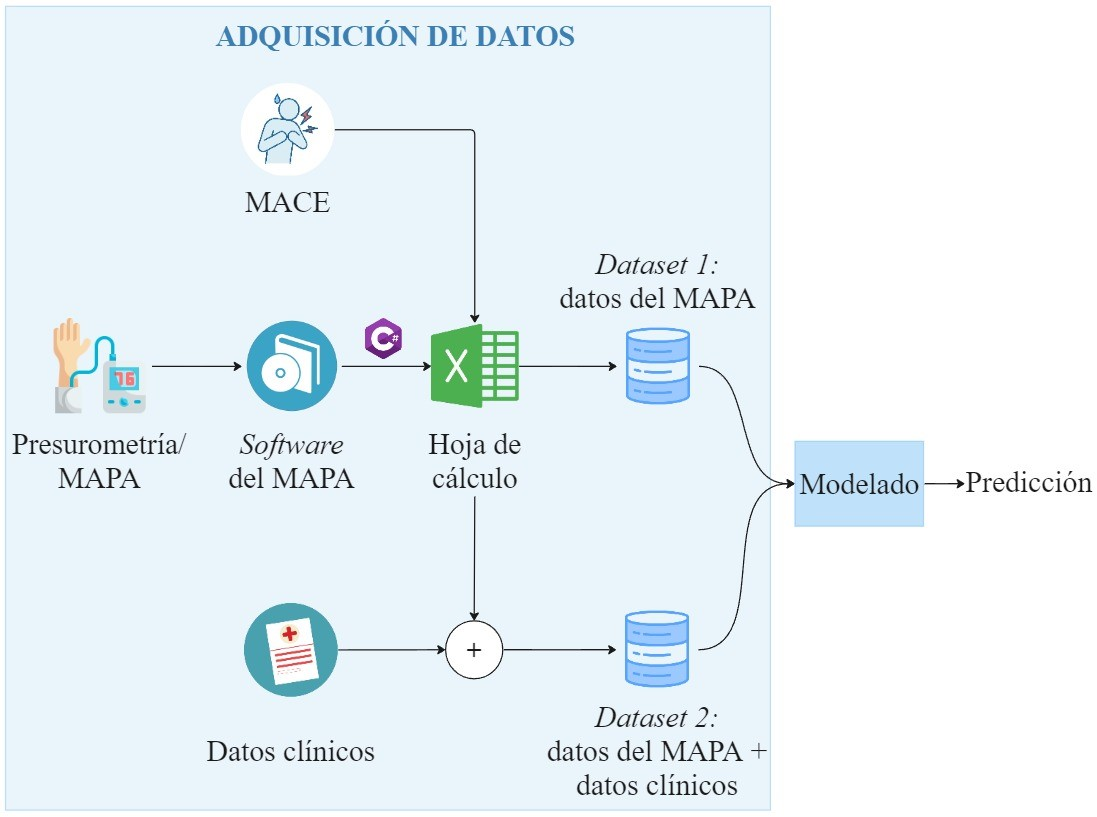
\includegraphics[width=\textwidth]{./Figures/adquisicion_datos2.jpg}
	\caption{Representación esquemática de las etapa de adquisición de datos.}\label{fig:adquisicion_datos}
\end{figure}

El primer \emph{dataset} se compone exclusivamente de información recopilada de las 
presurometrías realizadas a los pacientes hipertensos a partir del año 2013. Luego 
de realizar un MAPA, los datos se almacenan en un \emph{software} especializado de 
los presurómetros. Posteriormente, se extraen utilizando un programa desarrollado 
en C\myhash, para ser registrados en una planilla de cálculo. Sumado a esto, se incluyó 
la variable a predecir (MACE) para cada paciente mediante un análisis exhaustivo 
de su historial clínico. Especificamente, se registró si el paciente experimentó 
un accidente cerebrovascular no fatal, infarto agudo de miocardio, insuficiencia 
cardíaca, insuficiencia renal crónica o muerte.

Por otro lado, el segundo conjunto de datos contiene información adicional obtenida 
del historial clínico de cada paciente. Estos datos clínicos se agregan a la misma 
hoja de cálculo mencionada anteriormente, complementando así la información proveniente 
de las presurometrías.

El objetivo de utilizar dos \emph{datasets} es evaluar la calidad de los datos de 
las presurometrías para generar inferencias de manera independiente. En otras palabras, 
se buscó determinar en qué medida los datos del MAPA pueden ser utilizados por sí solos 
para obtener predicciones significativas y precisas de MACE. Al mismo tiempo, se procuró 
evaluar si la incorporación de información clínica contribuye a un mejor desempeño del 
modelo en términos de tasa de falsos negativos, AUC y otras métricas relevantes.



%----------------------------------------------------------------------------------------
%	ANALISIS EXPLORATORIO DE DATOS
%----------------------------------------------------------------------------------------
\section{Análisis exploratorio de datos}
 